\documentclass[varwidth=true, border=2pt]{standalone}

\usepackage{pgfplots}
\usepackage{tikz}
\usetikzlibrary{patterns}

% defining the new dimensions and parameters
\newlength{\hatchspread}
\newlength{\hatchthickness}
\newlength{\hatchshift}
\newcommand{\hatchcolor}{}
% declaring the keys in tikz
\tikzset{hatchspread/.code={\setlength{\hatchspread}{#1}},
         hatchthickness/.code={\setlength{\hatchthickness}{#1}},
         hatchshift/.code={\setlength{\hatchshift}{#1}},% must be >= 0
         hatchcolor/.code={\renewcommand{\hatchcolor}{#1}}}
% setting the default values
\tikzset{hatchspread=6pt,
         hatchthickness=0.4pt,
         hatchshift=0pt,% must be >= 0
         hatchcolor=black}
% declaring the pattern
\pgfdeclarepatternformonly[\hatchspread,\hatchthickness,\hatchshift,\hatchcolor]% variables
   {custom north west lines}% name
   {\pgfqpoint{\dimexpr-2\hatchthickness}{\dimexpr-2\hatchthickness}}% lower left corner
   {\pgfqpoint{\dimexpr\hatchspread+2\hatchthickness}{\dimexpr\hatchspread+2\hatchthickness}}% upper right corner
   {\pgfqpoint{\dimexpr\hatchspread}{\dimexpr\hatchspread}}% tile size
   {% shape description
    \pgfsetlinewidth{\hatchthickness}
    \pgfpathmoveto{\pgfqpoint{0pt}{\dimexpr\hatchspread+\hatchshift}}
    \pgfpathlineto{\pgfqpoint{\dimexpr\hatchspread+0.15pt+\hatchshift}{-0.15pt}}
    \ifdim \hatchshift > 0pt
      \pgfpathmoveto{\pgfqpoint{0pt}{\hatchshift}}
      \pgfpathlineto{\pgfqpoint{\dimexpr0.15pt+\hatchshift}{-0.15pt}}
    \fi
    \pgfsetstrokecolor{\hatchcolor}
%    \pgfsetdash{{1pt}{1pt}}{0pt}% dashing cannot work correctly in all situation this way
    \pgfusepath{stroke}
   }

\begin{document}
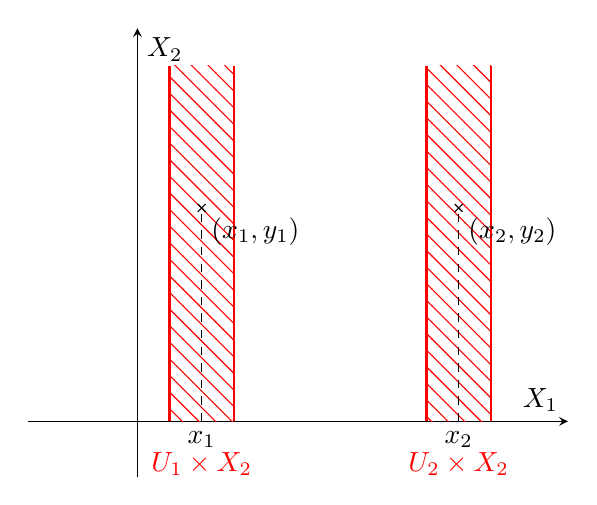
\begin{tikzpicture}
    \begin{axis}[
        legend pos=south west,
        axis x line=middle,
        axis y line=middle,
        %grid = major,
        %width=9cm,
        %height=4.5cm,
        grid style={dashed, gray!30},
        xmin=-1,     % start the diagram at this x-coordinate
        xmax= 6,    % end   the diagram at this x-coordinate
        ymin=-0.25,     % start the diagram at this y-coordinate
        ymax= 5,   % end   the diagram at this y-coordinate
        axis background/.style={fill=white},
        xlabel=$X_1$,
        ylabel=$X_2$,
        %xticklabels={,,},
        %yticklabels={,,},
        %xtick={-1,0,1,2,3,4,5},
        %ytick={-1,0,1,2,3,4,5},
        ticks=none,
        %tick align=outside,
        enlargelimits=true,
        tension=0.08]
        \addplot[hatchcolor=red,mark=none, pattern=custom north west lines, draw=none] coordinates {(0.5, 0) (0.5,5) (1.5,5) (1.5,0) };
        \addplot[red,mark=none, thick] coordinates {(0.5, 0) (0.5,5)};
        \addplot[red,mark=none, thick] coordinates {(1.5, 0) (1.5,5)};

        \addplot[hatchcolor=red,mark=none, pattern=custom north west lines, draw=none] coordinates {(4.5, 0) (4.5,5) (5.5,5) (5.5,0) };
        \addplot[red,mark=none, thick] coordinates {(4.5, 0) (4.5,5)};
        \addplot[red,mark=none, thick] coordinates {(5.5, 0) (5.5,5)};


        \addplot[mark=none, dashed] coordinates {(1, 0) (1,3)};
        \addplot[mark=none, dashed] coordinates {(5, 0) (5,3)};

        \addplot[mark=x] coordinates {(1, 3)};
        \addplot[mark=x] coordinates {(5, 3)};
        \node at (axis cs:1,3) [anchor=north west] {$(x_1, y_1)$};
        \node at (axis cs:5,3) [anchor=north west] {$(x_2, y_2)$};

        \node at (axis cs:1,0) [anchor=north] {$x_1$};
        \node at (axis cs:5,0) [anchor=north] {$x_2$};

        \node[red] at (axis cs:1,-0.3) [anchor=north] {$U_1 \times X_2$};
        \node[red] at (axis cs:5,-0.3) [anchor=north] {$U_2 \times X_2$};
    \end{axis}
\end{tikzpicture}
\end{document}
